\documentclass{beamer}
\usetheme[pageofpages=of,% String used between the current page and the
                         % total page count.
          bullet=circle,% Use circles instead of squares for bullets.
          titleline=true,% Show a line below the frame title.
          alternativetitlepage=true,% Use the fancy title page.
       %   titlepagelogo=logo-polito,% Logo for the first page.
       %   watermark=watermark-polito,% Watermark used in every page.
       %   watermarkheight=100px,% Height of the watermark.
       %   watermarkheightmult=4,% The watermark image is 4 times bigger
                                % than watermarkheight.
          ]{Torino}

\setbeamertemplate{footline}{
  \begin{beamercolorbox}[wd=\paperwidth,ht=1ex,dp=1ex]{footline}
    \vspace{5pt} \hspace{1em} \insertframenumber/\inserttotalframenumber
  \end{beamercolorbox}
}

\newcommand{\given}{\,|\,}
\newcommand{\balpha}{\boldsymbol{\alpha}}
\newcommand{\bmu}{\boldsymbol{\mu}}

\usepackage{colortbl}
\definecolor{LightGray}{gray}{0.9}
\definecolor{DarkGray}{gray}{0.3}
\definecolor{LightCyan}{rgb}{0.9, 1, 1}
\definecolor{LightRed}{rgb}{1, 0.8, 0.8}
\definecolor{LightGreen}{rgb}{0.8, 1, 0.8}
\definecolor{DarkGreen}{rgb}{0.3, 0.5, 0.3}



\author{Brendon J. Brewer}
\title{Introduction to Bayesian Statistics}
\institute{Summer Institute in Statistical Genomics \\
The University of Auckland, November 2026}
\date{}


\linespread{1.3}
\usepackage{minted}
\usepackage[utf8]{inputenc}
\usepackage{dsfont}


\begin{document}

\frame{\titlepage}


\begin{frame}
\centering
\Large
Posterior Predictive Checks

\end{frame}


\begin{frame}
\frametitle{The Good News}
\begin{itemize}
\item Bayesian statistics always works...\pause
\item {\bf If} your prior beliefs are well described by the prior,
and your knowledge of how the data and parameters are related is well described
by the sampling distribution.\pause
\item Also you need to be able to do the calculations :-)
\end{itemize}


\end{frame}


\begin{frame}
\frametitle{The Bad News}
\begin{itemize}
\item For silly choices of prior and/or likelihood, it is possible to get
a silly posterior distribution. It is not always obvious that a particular choice
is silly (in a way that matters).\pause
\item In practice, choices are often based on convenience and tradition.
\end{itemize}


\end{frame}


\begin{frame}
\frametitle{Spherical Cow in a Vacuum}
\url{https://en.wikipedia.org/wiki/Spherical_cow}

\begin{center}

\includegraphics[width=0.4\textwidth]{images/spherical_cow.png}

Credit: Ingrid Kallick (\url{http://www.ikallick.com/})
\end{center}


\end{frame}



\begin{frame}
\frametitle{Simple Linear Regression Example}
We will use a simple linear regression example to illustrate the idea
of {\bf posterior predictive checks}, which are used to get some insight into
the model assumptions being used.

\end{frame}


\begin{frame}
\frametitle{Simple Linear Regression: Fake Data}
I will generate some data from the curved relationship:
\begin{align}
y_i &= \beta_0 + \beta_1 x_i + \beta_2 x_i^2 + \epsilon_i\\
\epsilon_i \given \sigma &\sim \textnormal{Normal}(0, \sigma^2)
\end{align}

\pause

But we will fit the data without the quadratic term.


\end{frame}

\begin{frame}[fragile]
\frametitle{Simple Linear Regression: Fake Data}
\begin{minted}{r}
set.seed(123)
x = seq(-3, 3, length=100)
y = 1 + x + x^2 + rnorm(length(x))

data = data.frame(x=x, y=y)
write.csv(data, "quadratic_data.csv", row.names=FALSE)
\end{minted}

\end{frame}


\begin{frame}
\frametitle{Simple Linear Regression: Fake Data}

\begin{center}
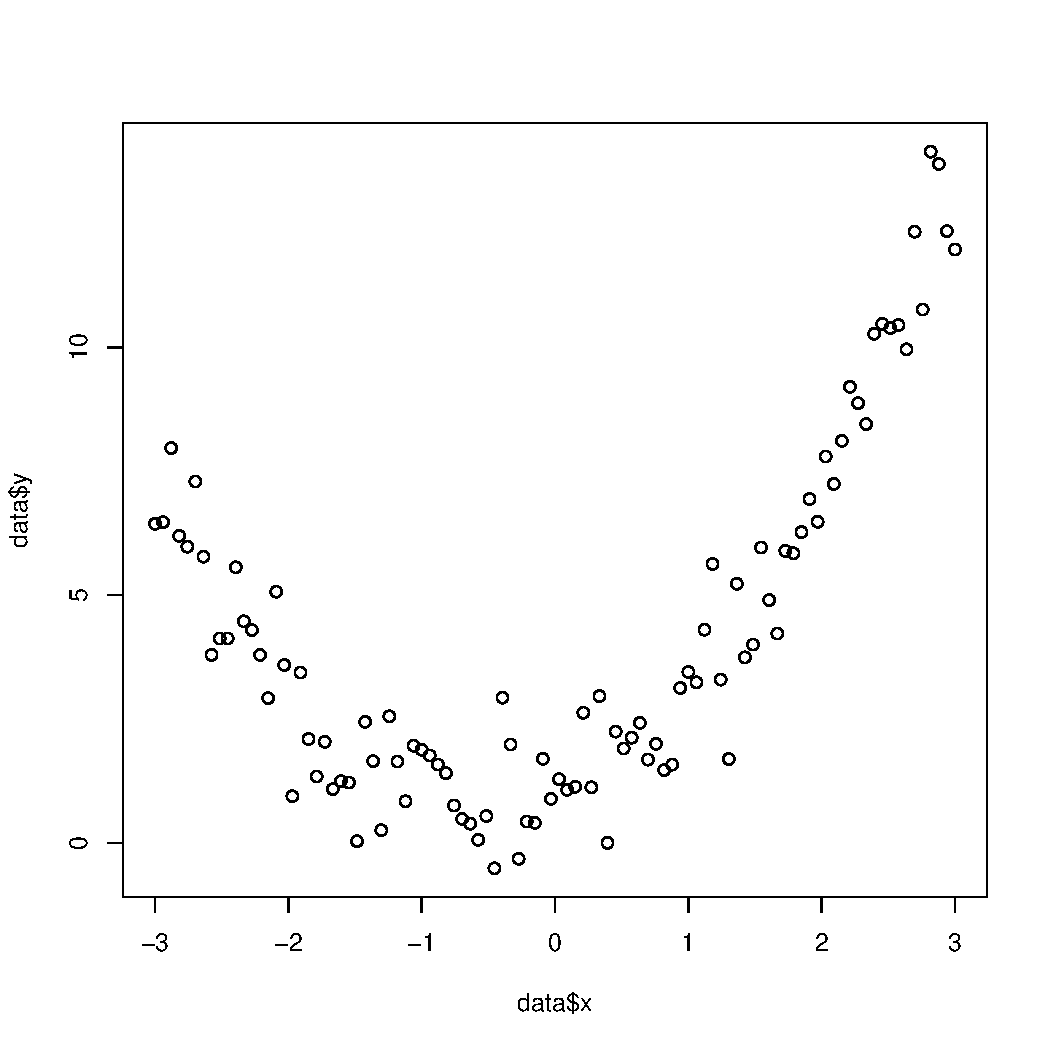
\includegraphics[width=0.6\textwidth]{images/quadratic_data.pdf}
\end{center}

\end{frame}


\begin{frame}
\frametitle{Common Sense}
By looking at the data, you can tell that a linear fit is probably not a good
idea. {\bf Food for Thought}: Does looking at the data to help decide what
model to fit violate any Bayesian principles?


\end{frame}


\begin{frame}[fragile]
\frametitle{Simple Linear Regression: JAGS Model}
\footnotesize
\begin{minted}{r}
model
{
    beta0 ~ dunif(-1000, 1000)
    beta1 ~ dunif(-1000, 1000)
    log_sigma ~ dunif(-10, 10)
    sigma <- exp(log_sigma)

    for(i in 1:length(y))
    {
        mu[i] <- beta0 + beta1*(x[i] - mean(x))
        y[i] ~ dnorm(mu[i], 1/sigma^2)
    }
}
\end{minted}

\end{frame}



\begin{frame}[fragile]
\frametitle{Residuals}

\begin{itemize}
\item When doing classical linear regression, you get a single best-fit line.
Subtracting it from the data gives you {\bf residuals}.\pause
\item We can do the same here, except we won't have a single set of residuals
because we don't get just one best-fit line.\pause
\item The residuals are supposed to look like noise. {\bf Note}: The prior
distribution of the residuals is iid Normal but the posterior is far from this!
\end{itemize}

\end{frame}

\begin{frame}
\frametitle{Simple Linear Regression: Lines Through Data}

\begin{center}
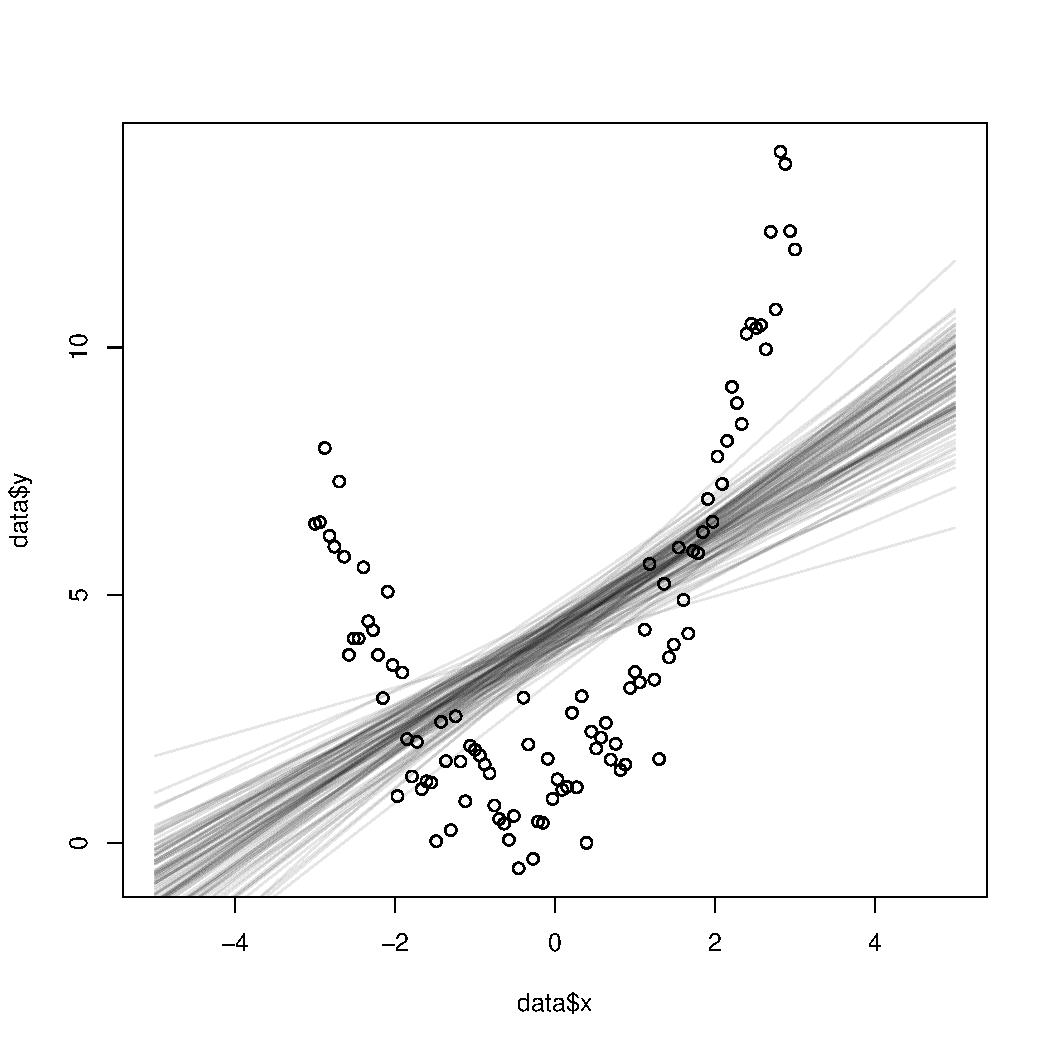
\includegraphics[width=0.6\textwidth]{images/quadratic_fit.pdf}
\end{center}

\end{frame}


\begin{frame}[fragile]
\frametitle{Residuals}

\begin{itemize}
\item Looking at residuals is useful as it can tell you in what particular ways
your model might be wrong.\pause
\item It is slightly harder to look at residuals when you have a whole
distribution of them, but you can plot the residuals once per posterior sample
(and make a movie!).\pause
\item However, residuals are only usually possible if the model has something like
\mintinline{r}{y[i] ~ dnorm(mu[i], 1/sigma^2)} in it. What if it doesn't?
\end{itemize}

\end{frame}


\begin{frame}
\frametitle{Posterior Predictive Checks}

    \begin{columns} % Create two columns
        \column{0.5\textwidth} % Left column (50% width)
        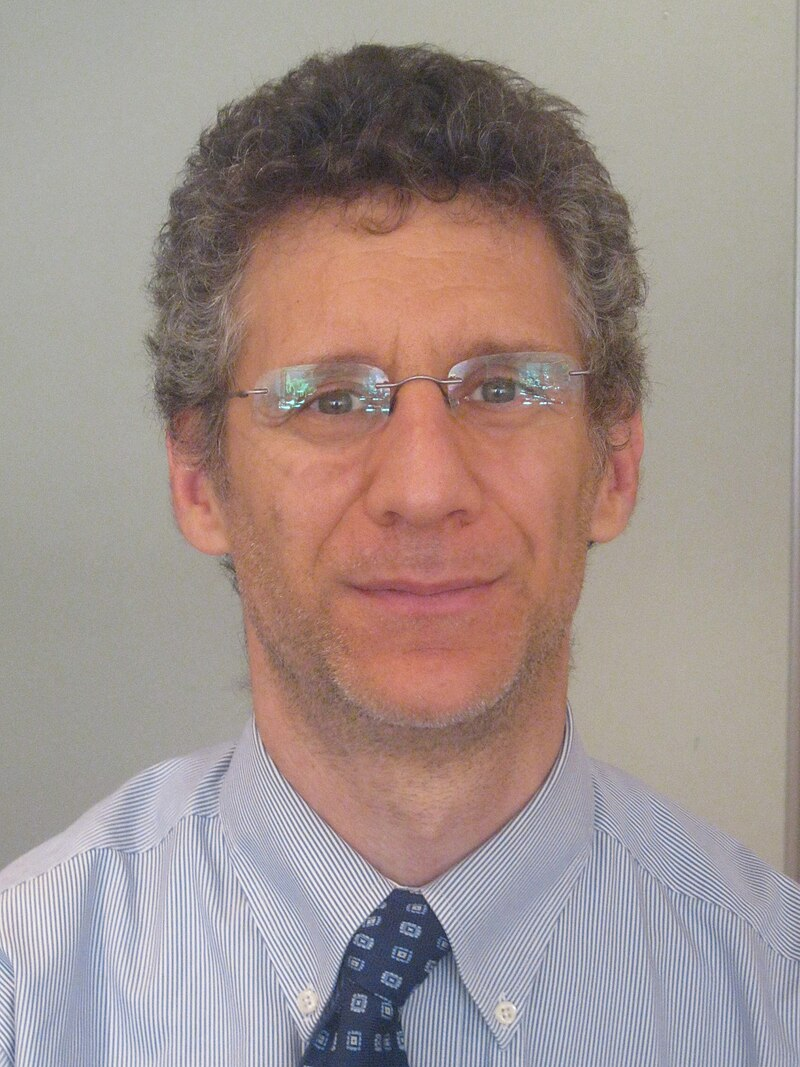
\includegraphics[width=0.8\linewidth]{images/gelman.jpg}

        \column{0.5\textwidth} % Right column (50% width)
        Well-known US statistician Andrew Gelman is a fan of posterior
        predictive checks.
     \end{columns}

\end{frame}


\begin{frame}
\frametitle{Posterior Predictive Checks}
\begin{itemize}
\item These are not derived from probability theory --- so are not strictly
Bayesian --- but they help you understand your model better.\pause
\item Take the posterior distribution for the parameters and use it to predict
{\bf a whole new dataset} just like the original dataset.\pause
\item If the model is `good', the real data should resemble the simulated
data --- you shouldn't be able to pick out the real data from a lineup.
\end{itemize}
\end{frame}


\begin{frame}[fragile]
\frametitle{Simulating New Data in JAGS}
This is like simulating one new data point, except we are putting the
prediction nodes inside the loop (so we get a whole dataset).

\begin{minted}{r}
for(i in 1:length(y))
{
    mu[i] <- beta0 + beta1*(x[i] - mean(x))
    y[i] ~ dnorm(mu[i], 1/sigma^2)
    y_new[i] ~ dnorm(mu[i], 1/sigma^2)
}
\end{minted}

\end{frame}

\begin{frame}[fragile]
\frametitle{Simulating New Data in JAGS}
Some practical tips:\pause
\begin{itemize}
\item Since a single dataset might be large, and you are generating a whole
lot of datasets, you might want to use a lot of thinning.\pause
\item To make it easier to deal with the output, monitoring {\em only}
\mintinline{r}{y_new} might be a good idea.
\end{itemize}

\end{frame}


\begin{frame}[fragile]
\frametitle{Simulating New Data in JAGS}
JAGS knows the difference between \mintinline{r}{y} (the real data)
and \mintinline{r}{y_new} (the simulated data), because we provided it with
values for \mintinline{r}{y} in the data, but not \mintinline{r}{y_new}.

\end{frame}


\begin{frame}[fragile]
\frametitle{Lineup of Datasets}

\begin{center}
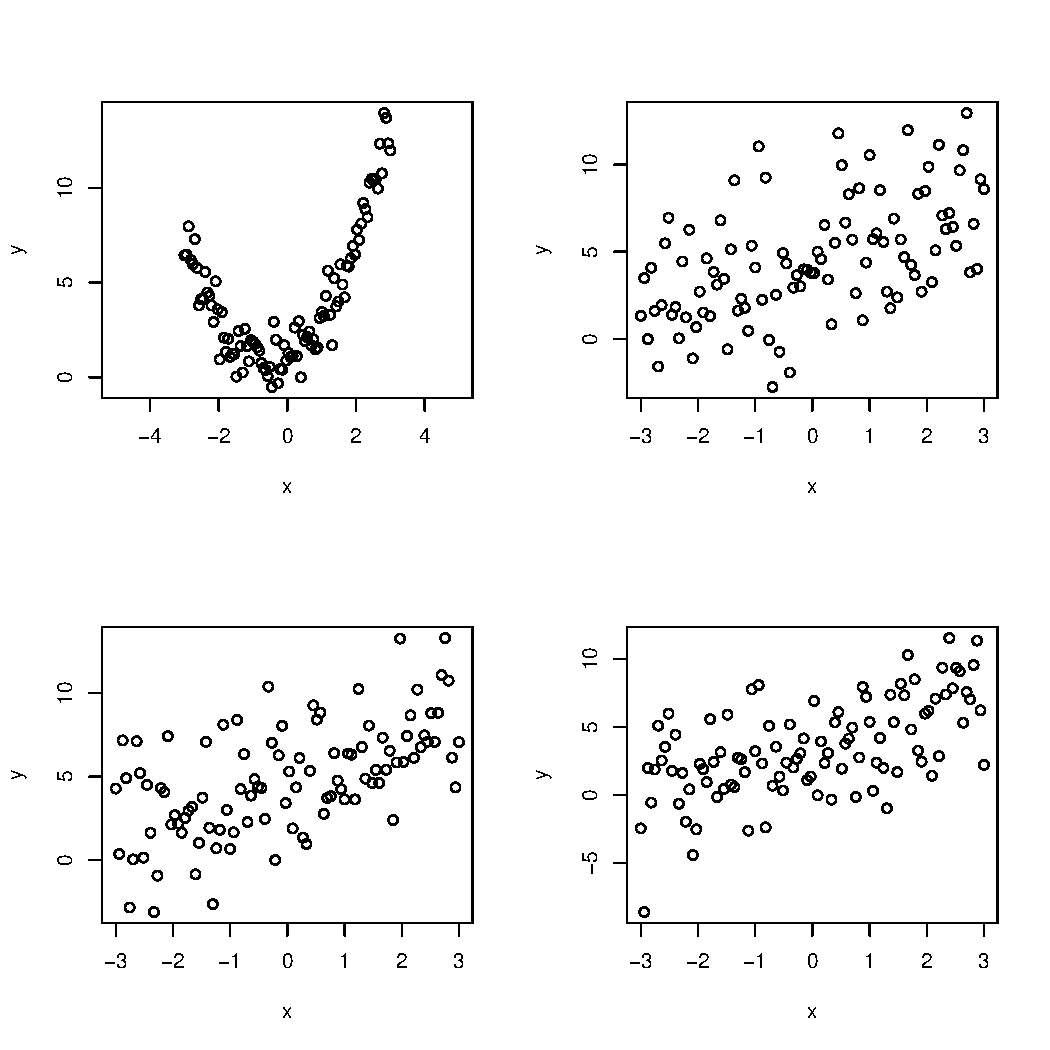
\includegraphics[width=0.6\textwidth]{images/quadratic_lineup.pdf}
\end{center}


\end{frame}


\begin{frame}[fragile]
\frametitle{Lineup of Datasets}
In this example, we can clearly distinguish the real dataset from the
fake datasets. The real data set is {\em atypical} of the probability
distribution over datasets, so the posterior predictive check is failed.\\[0.5em]\pause

Some people would do a formal (classical) hypothesis test of the null hypothesis
that the true data is `drawn from' the distribution over datasets. In STATS 331
we will stick to informal checks by making plots of the simulated datasets.

\end{frame}


\begin{frame}[fragile]
\frametitle{Philosophy}
In the Bayesian framework, the correct way to assess the quality of a model
is to calculate the marginal likelihood and do model comparison against an
alternative model. Usually, in the same situation where a PPC would be failed,
you would also get a low marginal likelihood.\\[0.5em]\pause

Posterior predictive checks can give you a good idea of what an alternative
model should look like.

\end{frame}



\begin{frame}[fragile]
\frametitle{Philosophy}
\begin{itemize}
\item Passing a PPC is no guarantee that your inferences are good.\pause
\item Failing a PPC is no guarantee that your inferences are bad.\pause
\item This does not make them pointless --- they help you to understand
your model, and prevent you from building in unintentional bad assumptions.
\end{itemize}
\end{frame}

\begin{frame}[fragile]
\frametitle{Example From My Research}
Measurements of the magnitude (brightness) of pairs of images of gravitationally
lensed quasars. Can you tell which is the real dataset?

\end{frame}

\begin{frame}[fragile]
\frametitle{Example From My Research}

\begin{center}
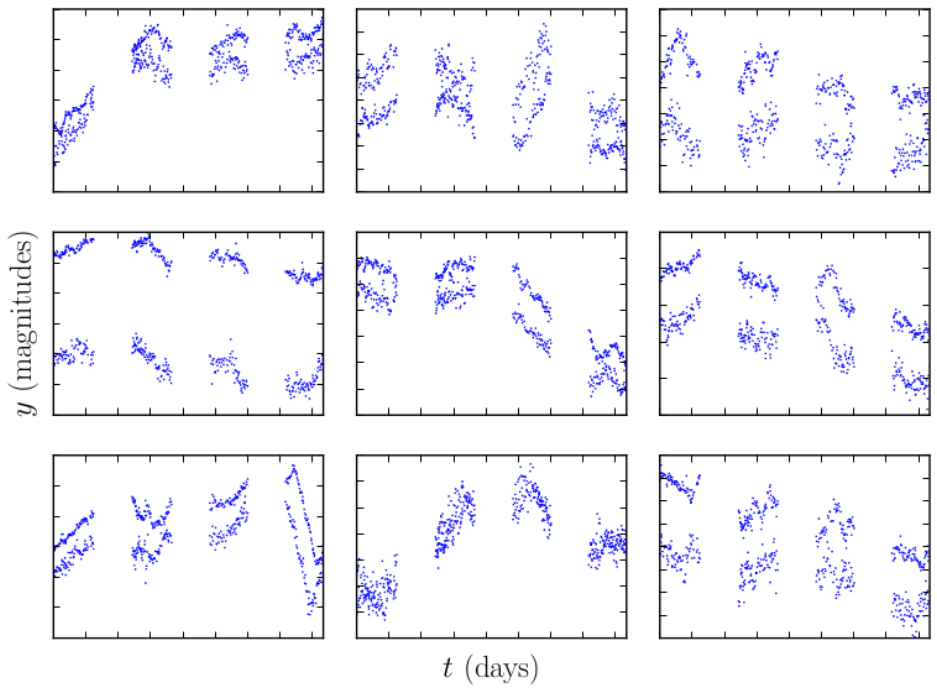
\includegraphics[width=0.7\textwidth]{images/time_delays.png}
\end{center}

\end{frame}



\end{document}

